

Si basa sul giudizio, e soprattutto su informazioni a contorno. Si perde la rappresentatività del campione statistico, ma ci troverà delle evidenze su ciò che staremo cercando.

\subsubsection{Difference Estimation Sampling}

Problemi tipici che bisogna indirizzare è la media e la deviazione standard.
La media non è un fenomeno che cattura bene l'andamento generale, per la presenza di \textit{outlier}, ovvero dei punti fuori dall'intervallo di rappresentazione. %?
La media è quindi un parametro assolutamente inaffidabile (va verificato ulteriormente!). Un parametro più affidabile che non è soggetto agli \textit{outlier} è la mediana.

L'intervallo di confidenza è la probabilità che il campione rappresenti la parte della popolazione. Viene rappresentato con un $\epsilon$, e più piccolo è e meglio è. Solitamente, si usa un intervallo di confidenza del 90\%. Il problema è la possibilità di usare una distribuzione fallace completamente duale rispetto all'intervallo di confidenza.


\subsubsection{Tipi di campionamento}

\paragraph*{Campionamento Stop-or-Go} facciamo un campionamento ridotto, se non si trova ciò che cerco mi fermo.

\paragraph*{Campionamento discovery} usato quando l'occorrenza dell'evento che sto cercando è molto rara.

\paragraph*{Campionamento degli attributi} un attributo è qualsiasi caratteristica che identifica una transazione rispetto alle altre. Per esempio transazioni effettuate ad un certo orario.

\subparagraph*{Tasso di errore tollerabile} il massimo rate di errore tollerabile.

\paragraph*{Campionamento variabile} quanto è accurato il campione nel matchare l'intera popolazione? 


\subsubsection{Campionamento variabile}
Si guardi la figura \ref{fig:variable:sampling}.
\begin{figure}[h!]
	\begin{center}
		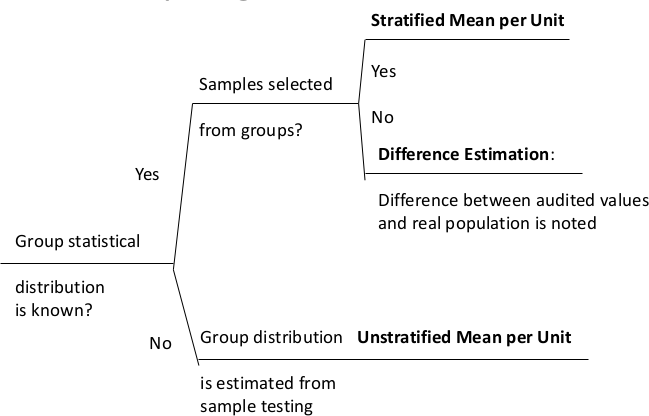
\includegraphics[scale=0.45]{res/img/variable_sampling.png}
	\end{center}
	\caption{Procedimento per il campionamento variabile.}
	\label{fig:variable:sampling}
\end{figure}



\paragraph{Generalized Audit Software}

Questa tipologia di tool sono molto utili, e danno la possibilità di avere accesso a:
\begin{itemize}
\item Accesso ai file
\item Organizzazione dei file
\item Selezione dei dati: selezione di un insieme di record
\item Funzioni statistiche
\item Funzioni aritmetiche
\end{itemize}

\subsection{Step 8: Preparare il rapporto di Audit}

È importante identificare:
\begin{itemize}
\item Chi deve ricevere il rapporto?
\item Contesto (cosa viene analizzato), gli obiettivi, il periodo coperto e quanto l'audit è durato\footnote{Audit che durano troppo poco con tante persone da analizzare non vanno bene, soprattutto se devono essere svolti in poco tempo.}.
\item Findings (quello che è stato trovato), che deve essere supportato da delle \emph{evidence} (prove). Le raccomandazioni possono essere date in due modi: seguendo gli standard (es. standard ISO) o facendo il merge tra la nostra esperienza, la nostra conoscenza e quello che può fare l'azienda per risolvere i problemi evidenziati.
\item Raggruppare per concretezza delle evidenze che abbiamo trovato.
\item menzionare i problemi trovati e le critiche costruttive.
\end{itemize}

Il rapporto di audit è una parte molto importante: un rapporto dettagliato permette ai successori di verificare il corretto funzionamento o meno dell'azienda negli anni passati, e permette di capire meglio il contesto. Un rapporto di audit dovrebbe essere bilanciato, altrimenti se si arriva a mettere a fuoco troppe cose negative non va bene, ma è importante anche non trascurarle. È importante tenere a mente che il rapporto di audit è fatto per essere letto dai ``piani alti''. Tenersi all'evidenze e ai fatti è sempre un'azione consigliata.



\todo{Inserire tabellina con un esempio di Report di un audit (facoltativo)}



\subsubsection{Evidenza}

Sono delle prove, e esistono in diverse forme:
\begin{itemize}
\item Note dalle interviste
\item Risultati dei test

Le migliori fonti per ottenere informazioni sono:
\begin{itemize}
\item Esterne: fonti da organizzazioni esterne (per esempio i fornitori).
\item Qualificate: le più autoritative
\item Oggettive: evidenze per cui non è possibile esprimer
\item Email o corrispondenza
\item Documentazione
\item Osservazioni
\end{itemize}e un periodo soggettivo
\item Tempo: deve essere coerente con la nostra attività di audit 
\end{itemize}



\subsubsection{Comunicazione dei risultati}

La comunicazione dei risultati è una passo decisivo. Questi risultati devono essere riportati alle persone interessate.
La parte grossa dell'audit deve essere consegnata ai manager ad alto livello.\todo{Copia schema?}


\subsection{Step 9: Prosieguo}


Il \textit{follow-up} serve \todo{boh}

\section{Raccomandazioni finali sull'Audit}

Queste ultime note sono molto importanti e vanno sempre tenute in considerazione:
\begin{itemize}
\item Mai eccedere lo scopo di quello che si deve fare, ovvero, mai ficcare il naso dove non serve. I permessi che vengono accordati devono essere messi per iscritto, affinchè ne rimanga una traccia.
\item Tutti i test potrebbero impattare sul sistema, ed è quindi una buona pratica avvisare i settori interessati dei possibili disguidi prima di iniziare ad eseguire qualisiasi test.
\item Quando si lavora con i dati è importante non toccare dati o configurazioni importanti.
\end{itemize}


\section{Tipi di audit}

Audit finanziario, operazionale, integrativo, forense (è successo un evento negativo che ha scatenato reazioni civili o penali e viene chiamato un auditor esterno per fare analisi forense), IS, amministrativo.

\subsubsection{Computer-Assisted Audit Techniques (CAAT)}

I software permettono agli auditor di:
\begin{itemize}
\item Accedere e analizzare i dati nel database
\item Effettuare test di compliance
\item Effettuare penetration test
\item Testare le applicazioni
\end{itemize}


\subsubsection{Control self-assignment}
I benefici consistono nel fatto che si lavora con le persone e questo serve per dare un segnale, ovvero che si aiuta a dare una migliore impressione dell'azienda.



\subsubsection{Service Learning Component: Non-Disclosure Agreement}

Supponiamo che si sia una situazione del genere:

\begin{verbatim}
You: I developed an audit plan for Help-The-Community
Interviewer: What specifically did you do?
You: We tried to break into their wireless network
Interviewer: What did you find?
You: They had no security. They were hopelessly non-technical.
Their password was `HelpTheCommunity', and transmissions were
unencrypted. I could read everything...
\end{verbatim}

In questo dialogo, è evidente come ci sia un rilascio di informazioni non controllato, che potrebbe portare un attacco di tipo malizioso.





Il problema è che l'intervistato ha divulgato informazioni sull'azienda, nonostante l'NDA. Anche se i problemi fossero attualmente risolti sta comunque infangando il nome della società auditata.


Bisognerebbe invece dire:
\begin{verbatim}
You: I developed an audit plan for Help-The-Community
Interviewer: What specifically did you do?
You: We did a penetration test. However, I signed a
non-disclosure agreement, so I am not at liberty to
say specifically what we did or found.
Interviewer: Were you successful in breaking in?
You: I can't say. However, if you would like to contact my
community partner as a reference, here is her contact
information...
\end{verbatim}



%ESERCIZI

The primary purpose of generalized audit software (GAS) is to:
\begin{itemize}
\item Find fraudulent transactions
\item Determine sample mean compared to population mean
\item Extract data for a Substantive Test (risposta esatta)
\item Organize an audit report
\end{itemize}


% Altro esercizio

A compensating control is defined as:
\begin{itemize}
\item Two strong controls address the same fault
\item A fault is addressed by a weak control and strong control in another area (risposta esatta)
\item A control addresses a specific problem
\item A control that fixes the problem after it is detected
\end{itemize}


% Altro esercizio

An IS auditor should plan their audit approach based upon:

\begin{itemize}
\item Materiality
\item Management recommendations
\item ISACA recommendations
\item Risk (risposta esatta)
\end{itemize}

%Altro esercizio


A hash total is maintained on each batch file to ensre no transactions are lost. This is an example of a:
\begin{itemize}
\item Preventive Control
\item Detective Control (risposta esatta)
\item Compensating Control
\item Corrective Control
\end{itemize}


%Altro esercizio


The first step that an auditor should take is:
\begin{itemize}
\item Prepare the Audit Objectives and Scope
\item Learn about the organization (risposta corretta)
\item Study ISACA audit recommendations for the functional area
\item Perform a rusk assessment
\end{itemize}

%Altro esercizio

An audit that considers how financial information is generated from both a business process and IS handling side side is know as:
\begin{itemize}
\item Financial audit
\item Operational audit
\item Administrative audit
\item Integrated audit (risposta esatta)
\end{itemize}

%Altro esercizio

An auditor over-tests (tests a greater percent than actually exist) samples that are expected to be most risky:
\begin{itemize}
\item Variable Sampling
\item Attribute Sampling
\item Statistical Sampling
\item Non-statistical Sampling (risposta corretta)
\end{itemize}

%Altro esercizio

The possibility that a router does not catch spoofed IP addresses is known as a

\begin{itemize}
\item Inherent risk
\item Control risk (risposta corretta)
\item Detection risk
\item External risk
\end{itemize}

% RISCHIO DI CONTROLLO = QUANDO IL CONTROLLO FALLISCE -> Per mitigarlo si usano controlli compensativi

%Altro esercizio

Testing a firewall to ensure that it only permits web traffic intro the DMZ is known as

\begin{itemize}
\item Compliance Test (risposta corretta)
\item Substantive Test
\item Detection Test
\item Preventive Test
\end{itemize}

%Altro esercizio

An inherent risk for a school would be

\begin{itemize}
\item Students trying to hack into the system to change grades (risposta corretta)
\item A firewall does not catch spoofed IP addresses
\item An audit does not find fraud which actually exists
\item People do not change their passwords regularly
\end{itemize}

%Altro esercizio

